%
% File report.tex
%
%% Based on the style files for ACL 2018 and NAACL 2018, which were
%% Based on the style files for ACL-2015, with some improvements
%%  taken from the NAACL-2016 style
%% Based on the style files for ACL-2014, which were, in turn,
%% based on ACL-2013, ACL-2012, ACL-2011, ACL-2010, ACL-IJCNLP-2009,
%% EACL-2009, IJCNLP-2008...
%% Based on the style files for EACL 2006 by 
%%e.agirre@ehu.es or Sergi.Balari@uab.es
%% and that of ACL 08 by Joakim Nivre and Noah Smith

\documentclass[11pt,a4paper]{article}
\usepackage[hyperref]{naaclhlt2019}
\usepackage{times}
\usepackage{latexsym}
\usepackage{todonotes}
\usepackage{url}
\usepackage{units}

\aclfinalcopy % Uncomment this line for the final submission
%\def\aclpaperid{***} %  Enter the acl Paper ID here

%\setlength\titlebox{5cm}
% You can expand the titlebox if you need extra space
% to show all the authors. Please do not make the titlebox
% smaller than 5cm (the original size); we will check this
% in the camera-ready version and ask you to change it back.

\newcommand\BibTeX{B{\sc ib}\TeX}

\title{One Million Posts Corpus}

\author{Jens Becker \and Julius Plehn \and Oliver Pola \\ 
	Language Technology Group \\
	Fachbereich Informatik \\
	Fakultät für Mathematik, Informatik und Naturwissenschaften \\
	Universität Hamburg
}

\date{28.02.2020}

\begin{document}
\maketitle
\begin{abstract}
The purpose of this term paper is to summarize the development effort put into the creation of a multi-model neural network for category classification. This contains used preprocessing steps of the initial corpus, integration of an embedding layer and the actual deep learning network. Finally, an evaluation is given as well as ideas for future work. \todo{we conclude that...}

 
\end{abstract}

\section{Introduction}

Many work has been done on NLP tasks using English language.
To contribute to the knowledge about German language, similar work has been repeated on large collections of german text.
\newcite{Schabus17} produced and analyzed the \textit{One Million Posts Corpus} described in the next chapter in more detail. Later \newcite{Schabus18} improved their results using other methods.

Our work will use that corpus and tries to reproduce some of the original work.
The focus lies on applying the recurrent deep learning method LSTM~\cite{lstm}.

The corpus contains labelled data for multiple categories.
As the previous work did apply classifiers for each category on its own, we try to contribute another approach, using all categores at once.\\

Our code is publicly available on GitHub\footnote{Our code available at \url{https://github.com/oliver-pola/OneMillionPostsCorpus/}}.

\section{Corpus}
The corpus\footnote{Corpus available at \url{https://ofai.github.io/million-post-corpus/}} used stems from the Austrian newspaper \textit{DER STANDARD}\footnote{DER STANDARD \url{https://www.derstandard.at}} which contains posts that are labelled according to nine distinct categories. The posts have been written during a time period from 2015-2016 and contain 1 million unlabelled posts as well as 11,773 hand-labelled posts.


\subsection{Categories}
In Table~\ref{tab:categories} an overview of included categories is shown. The meaning of those categories is explained by~\newcite{Schabus17}.
In the first column is shown that for example 3599 posts were labbelled in the \textit{Off Topic} category. 
The second column shows that in this case 580 posts where indeed \textit{Off Topic}, resulting in 16\% of the labelled posts of this specific category. 

\begin{table}
	\centering\small
	\begin{tabular}{l r r r r r}
		& Labeled & \multicolumn{2}{c}{Does apply} & \multicolumn{2}{c}{We apply} \\
		\hline
		Sentiment Negative & 3599 & 1691 & 47\% \\
		Sentiment Neutral & 3599 & 1865 & 52\% \\
		Sentiment Positive & 3599 & 43 & 1\% \\
		Off Topic & 3599 & 580 & 16\% \\
		Inappropriate & 3599 & 303 & 8\%\\
		Discriminating & 3599 & 282 & 8\%\\
		Possibly Feedback & 6038 & 1301 & 22\% & 72 & 2\%\\
		Personal Stories & 9336 & 1625 & 17\% & 47 & 1\%\\
		Arguments Used & 3599 & 1022 & 28\%\\
	\end{tabular}
	\caption{Categories of posts and their distribution according to \newcite{Schabus17}}
	\label{tab:categories}
\end{table}

As previously mentioned there are 11,773 labelled posts. This means after labelling 3599 posts in each category, there were another 2439 posts labeled in the \textit{Possibly Feedback} and yet another 5737 posts in the \textit{Personal Stories} category only.
These additional posts were strongly biased towards positive labels, so that the category finally applies to 22\% / 17\% of posts, whereas in a random sample like the 3599 posts it is rather 2\% / 1\%.
Besides this questionable labelling method, the additional posts can't be used in our method for technical reasons.
As we want to build a model that is capable of identifying multiple categories at once we use only posts that are annotated as 0 or 1 for each category.
So only those 3599 posts can be used in our approach.  

Looking at the percentage where the categories do apply, it becomes already clear that most of them will be problematic. 
Having only a few positive labels will encourage the model to predict always negative, as this will result in a 99\% accuracy when the positive labels are 1\% only, like in the \textit{Sentiment Positive} category. With that small set of training data it is also not applicable to omit some of the negative posts to train with an artificial balance around 50\% each.

Also there is the \textit{Off Topic} category with probably enough positives, but technically we will consider single posts only, out of their context among other posts belonging to certain articles. But the latter would be necessary to detect something as off-topic.

To summarize, we expect to produce useful results only in the \textit{Sentiment Negative}, \textit{Sentiment Neutral} and \textit{Arguments Used} categories only.

\section{Embedding}

Embedding is the task to preproccess the textual input, our posts, to some numerical vectors that can be calculated with in a neural network. 
We use Word2Vec~\cite{word2vec}, where the high dimensionality of the resulting vector tries to encode the semantic of words. 
Words that often appear in similar context are considered to have similar meaning and appear in close distance in the resulting vector space.
Word2Vec is a learning task on its own that we do not perform but use a pretrained german model\footnote{German Word2Vec model available at \url{https://deepset.ai/german-word-embeddings}} that uses a vocabulary of 1,309,281 words, each embedded into a vector of size 300.
The model is loaded and applied by Gensim\footnote{Gensim \url{https://radimrehurek.com/gensim/}}~\cite{gensim}.

A post therefor is split into words and each word embedded into a vector. Having multiple words in a post results to a list of vectors or rather a matrix. 
Words not found in the vocabulary will be skipped in the process. 
Since a neural network expects a fixed input size (at least within one batch), the matrix is padded to the size 80$\times$300, cutting off too long posts and filling short ones with zeroes at the end. 
We chose the number 80 based on the maximum length of posts in the training data to be 161 and the average 37 words, also having memory and processing time in mind.

The standard approach applying such an embedding seems to be generating an embedding matrix, that contains the vectors for all the words in the vocabulary and then have the input to be the indices of the words. 
This matrix is then fed into the preprocessing layer of the network. With this approach we had some problems due to memory limitations on some systems. 
Also feeding the embedding matrix into the network and using Tensorflow on a GPU means to load that embedding matrix into the limited GPU memory. 
Many rows in that matrix will not be used in the current batch, some of them will in fact never be used.

Instead we considered the embedding as a preprocessing step, using Gensim to go from words to vectors directly.
The input of the network will then be vectors already and no embedding matrix needs to be stored in GPU memory.
Since we also do the preprocessing only once and then repeatedly feed the vectors into the network, the embedding is also done only once instead of embedding the same post again in each epoch.
Also this opens up the ability to free the memory of the embedding model after preprocessing is done.
That reduced the memory needs of our model and we could use less advanced hardware for training, only dealing with processing time.


\section{Deep Learning}

This chapter shows the implementation of our network model, justifies the chosen hyper parameters and describes the training.


\subsection{Model}
The model has been implemented using Tensorflow 2 and Keras. Because it tends to overfit several dropouts are applied. As can be seen in Figure~\ref{fig:model} the first layer uses a dropout rate of 20\%. The following LSTM layer uses 128 units while also applying a dropout rate of 40\%. The LSTM is wrapped by a bidirectional layer which improved the performance by using information of the past, as well of the future. Finally, two dense layers are used, where the last layer maps the output of the network to the nine categories shown earlier.

\begin{figure}[h!]
	\centering
	
\includegraphics[trim={1cm 19.5cm 5cm 3cm},clip,page=2, width=0.5\textwidth]{img/model}
	\caption{Applied deep learning network}
	\label{fig:model}
\end{figure}

This describes our final model, we call \textit{Multi-Model} where we use all the categories combined to a vector of size 9.
To reproduce the original work, we first implemented a classifier that was considering a single category only. 
This model we call \textit{Single-Model} and it is similar to Figure~\ref{fig:model} except having only one unit in the final classification layer.


\subsection{Hyper Parameters}

The hyper parameters of our model are justified by a search over a range of values, shown in Figure~\ref{fig:hyper_params}. 
We completed a full training with each set of parameters. Finally the best model measured by $F_1$ score on the validation set is applied. 
A first impression was that out model performs well in the \textit{Arguments Used} category, so we concentrated to optimize for that category.

The training results are evaluated on two different systems and averaged over a total of six runs. 
Not shown in Figure~\ref{fig:hyper_params} is data we've collected for 32 and 192 LSTM units as well, because these don't contribute to our conclusion. 
We have chosen 128 LSTM units (having this bidirectional results in 256 trainable parameters) and 64 dense units, because we consider that peak as more  
noticeable compared to the 160 LSTM curve, it had a smaller standard deviation and we preferred to have fewer parameters.

\begin{figure}[h!]
	\centering
	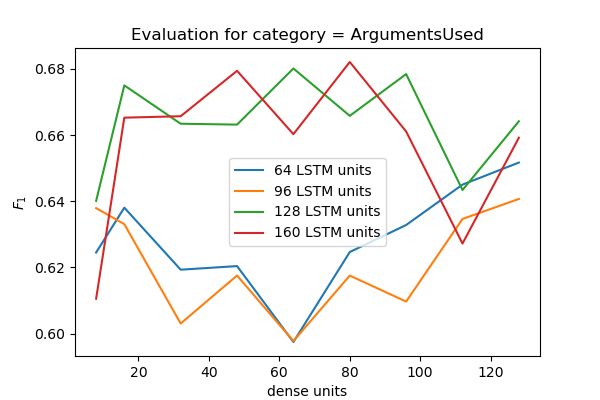
\includegraphics[trim={0.1cm 0cm 0.7cm 0.7cm},clip,width=0.5\textwidth]{img/training_meta}
	\caption{Search for best model based on different hyper parameters}
	\label{fig:hyper_params}
\end{figure}


\subsection{Training}

The dataset of 3599 fully labelled posts is split into a training set of 3059 posts and a validation set of 540 posts (15\%).

The training itself is supervised by using automatic learning rate adaptation (\textit{ReduceLROnPlateau}) and \textit{EarlyStopping}, which helps to reduce the overall training time.
Figure~\ref{fig:training_loss} shows the progress during training and the early stopping method applied, as training ends when validation loss starts to increase.

\begin{figure}[h!]
	\centering
	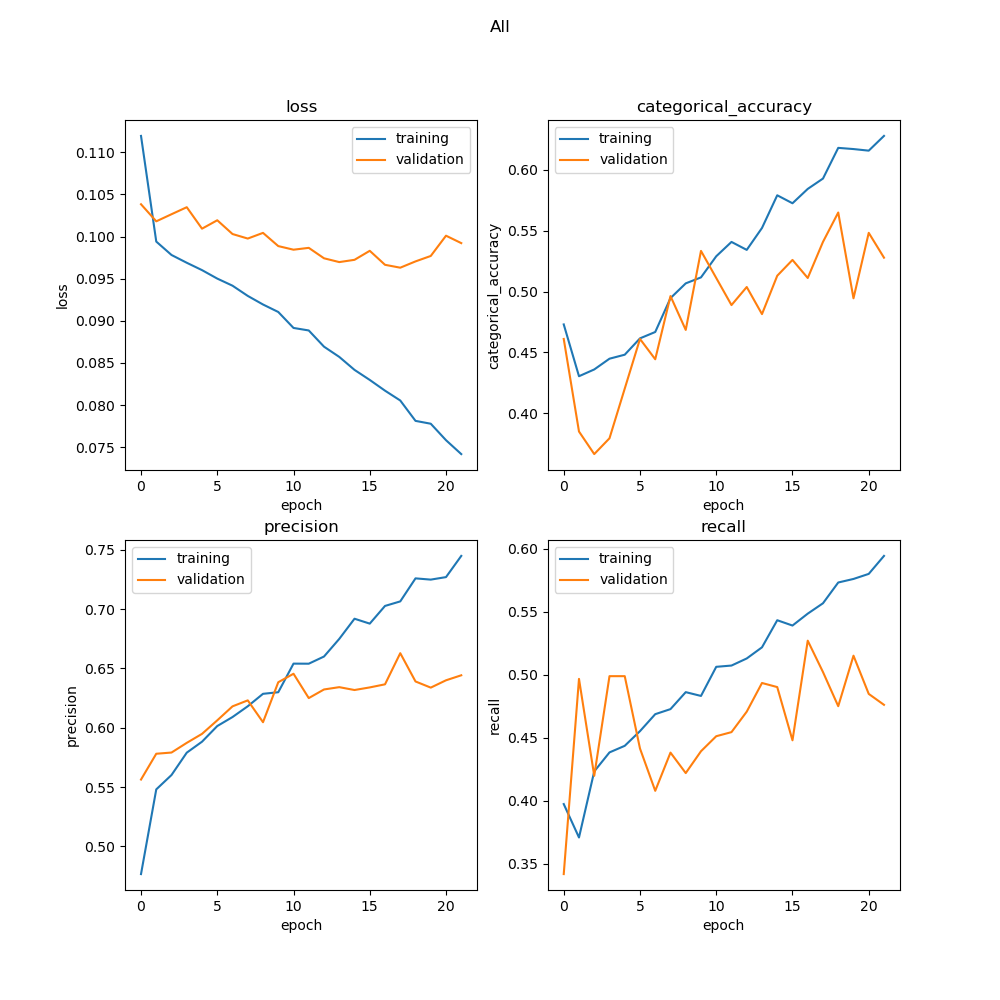
\includegraphics[trim={1.4cm 12.4cm 2cm 2.5cm},clip,width=0.5\textwidth]{img/training_All_22}
	\caption{Progress of loss function (left) and accuracy (right) during training}
	\label{fig:training_loss}
\end{figure}

The \textit{categorical accuracy} is shown in Figure~\ref{fig:training_loss} as summary over all categories. In fact it is the average of the accuracies in each category, weighted by the rate of positive labels. Later only accuracies for single categories, extracted from a vector of predictions, are analized.


\section{Results}
In this paragraph the performance of the models evaluated by \newcite{Schabus17} and us are compared.
While in Table~\ref{tab:results} all measurements of the single-model as well as the multi-model of every category is shown, a few categories are highlighted.

In Table~\ref{tab:results:sentiment_negative} the performance of our model classifying the category \textit{Sentiment Negative} is shown. As the corpus for this category is nearly equally balanced this is a good starting point for a comparison. While the precision of our single- as well as the multi-model is higher, the recall is much lower that the one described in the original paper. This therefore results in a lower $F_1$ score.
\begin{table}[h!]
	\centering\scriptsize
	\begin{tabular}{l r r r r r}
		& Accuracy & Precision & Recall & $F_1$ \\
		\hline
		Schabus et al. (best) & & 0.5842 & 0.7197 & 0.6137 \\
		Schabus et al. (LSTM) & & 0.5349 & 0.7197 & 0.6137 \\
		\hline
		Our Single-Model & 0.5630 & 0.5943 & 0.5142 & 0.5513\\
		Our Multi-Model & 0.6444 & 0.6550 & 0.4571 & 0.5384 \\
	\end{tabular}  
	\caption{Comparison: Sentiment Negative}
	\label{tab:results:sentiment_negative}
\end{table}

\begin{table*}
	\centering\small
	\begin{tabular}{l r r r r r r r r}
		& True Pos & True Neg & False Pos & False Neg & Accuracy & Precision & Recall & $F_1$ \\
		\hline
		Sentiment Negative & 145 & 159 & 99 & 137 & 0.56 & 0.59 & 0.51 & 0.55 \\
		& 112 & 236 & 59 & 133 & 0.64 & 0.65 & 0.46 & 0.54 \\
		\hline
		Sentiment Neutral & 190 & 133 & 149 & 68 & 0.60 & 0.56 & 0.74 & 0.64 \\
		& 216 & 124 & 126 & 74 & 0.63 & 0.63 & 0.75 & 0.68 \\
		\hline
		Sentiment Positive & 0 & 533 & 0 & 7 & 0.99 & 0 & 0 & 0 \\
		& 0 & 535 & 0 & 5 & 0.99 & 0 & 0 & 0 \\
		\hline
		Off Topic & 0 & 452 & 0 & 88 & 0.84 & 0 & 0 & 0 \\
		& 11 & 423 & 14 & 92 & 0.80 & 0.44 & 0.11 & 0.17 \\
		\hline
		Inappropriate & 0 & 504 & 0 & 36 & 0.93 & 0 & 0 & 0 \\
		& 1 & 483 & 0 & 56 & 0.90 & 1.00 & 0.02 & 0.03 \\
		\hline
		Discriminating & 0 & 497 & 0 & 43 & 0.92 & 0 & 0 & 0 \\
		& 1 & 492 & 3 & 44 & 0.91 & 0.25 & 0.02 & 0.04 \\
		\hline
		Possibly Feedback & 0 & 531 & 0 & 9 & 0.98 & 0 & 0 & 0 \\
		& 0 & 527 & 0 & 13 & 0.98 & 0 & 0 & 0 \\
		\hline
		Personal Stories & 0 & 532 & 0 & 8 & 0.99 & 0 & 0 & 0 \\
		& 0 & 534 & 0 & 6 & 0.99 & 0 & 0 & 0 \\
		\hline
		Arguments Used & 78 & 350 & 51 & 61 & 0.79 & 0.60 & 0.56 & 0.58\\
		& 99 & 339 & 41 & 61 & 0.81 & 0.71 & 0.62 & 0.66 \\
	\end{tabular}
	\caption{Comparison of the performance of the single- (top row in each category) vs the multi-model (bottom row)}
	\label{tab:results}
\end{table*}

Table~\ref{tab:results:sentiment_positive} is an example of the consequences of unbalanced data. While the accuracy is at around 99\% the precision, recall and $F_1$ score is zero. As the corpus only contains 1\% of positively labelled data for this category the model learns to predict always zero.
But the LSTM model in the original work had the exact same problem, while other models lead to non-zero but still unsatisfying scores.
\begin{table}[h!]
	\centering\scriptsize
	\begin{tabular}{l r r r r r}
		& Accuracy & Precision & Recall & $F_1$ \\
		\hline
		Schabus et al. (best) & & 0.2353 & 0.4651 & 0.1333 \\
		Schabus et al. (LSTM) & & 0 & 0 & 0\\
		\hline
		Our Single-Model & 0.9870 & 0 & 0 & 0 \\
		Our Multi-Model & 0.9907 & 0 & 0 & 0 \\
	\end{tabular}
	\caption{Comparison: Sentiment Positive}
	\label{tab:results:sentiment_positive}
\end{table}

Table~\ref{tab:results:arguments_used} shows the performance on the category \textit{Arguments Used}. In this case our multi-model LSTM outperforms the original model, as can be seen by comparing the $F_1$ score. This is especially noteworthy as this category is only applied positively in 28\% of the cases.  
\begin{table}[h!]
	\centering\scriptsize
	\begin{tabular}{l r r r r r}
		& Accuracy & Precision & Recall & $F_1$ \\
		\hline
		Schabus et al. (best) & & 0.6105 & 0.6614 & 0.6098 \\
		Schabus et al. (LSTM) & & 0.5685 & 0.6458 & 0.6047\\
		\hline
		Our Single-Model & 0.7926 & 0.6047 & 0.5612 & 0.5821 \\
		Our Multi-Model & 0.8111 & 0.7071 & 0.6188 & 0.6600 \\
	\end{tabular}
	\caption{Comparison: Arguments Used}
	\label{tab:results:arguments_used}
\end{table}


\section{Conclusion}

\todo{we conclude that...}


\bibliography{references}
\bibliographystyle{acl_natbib}
\appendix

%\section{Appendices}
%\label{sec:appendix}


\end{document}
